\section{数据分析与预处理}

在构建优化模型之前,对基础数据进行系统性的分析与处理是确保模型有效性的前提。本章旨在对该乡村的耕地结构、农作物种植现状及关键经济参数进行定量剖析,为后续模型提供必需参数,并洞察该农业系统的内在结构与潜在的经济驱动力。

\subsection{耕地资源与农学含义分析}

农业生产的边界首先由其拥有的土地资源所决定。该乡村的耕地由露天耕地与设施大棚两部分构成。如图\ref{fig:land_structure}所示,露天耕地总面积为1201亩,主要类型为梯田(52\%)与平旱地(30\%)。这种以旱作为主的土地结构,从农学角度揭示了该地区可能面临水资源约束和土壤保持的挑战,使得耐旱作物的选择和水土保持措施显得尤为重要。设施农业方面,16个普通大棚和4个智慧大棚共提供了12亩受控环境的耕作面积,为高附加值作物的生产提供了可能。这一系列的土地类型、面积及适种信息,将直接转化为优化模型中的地块面积参数$A_i$与种植适宜性参数$S_{ijk}$。

\begin{figure}[t]
	\centering
	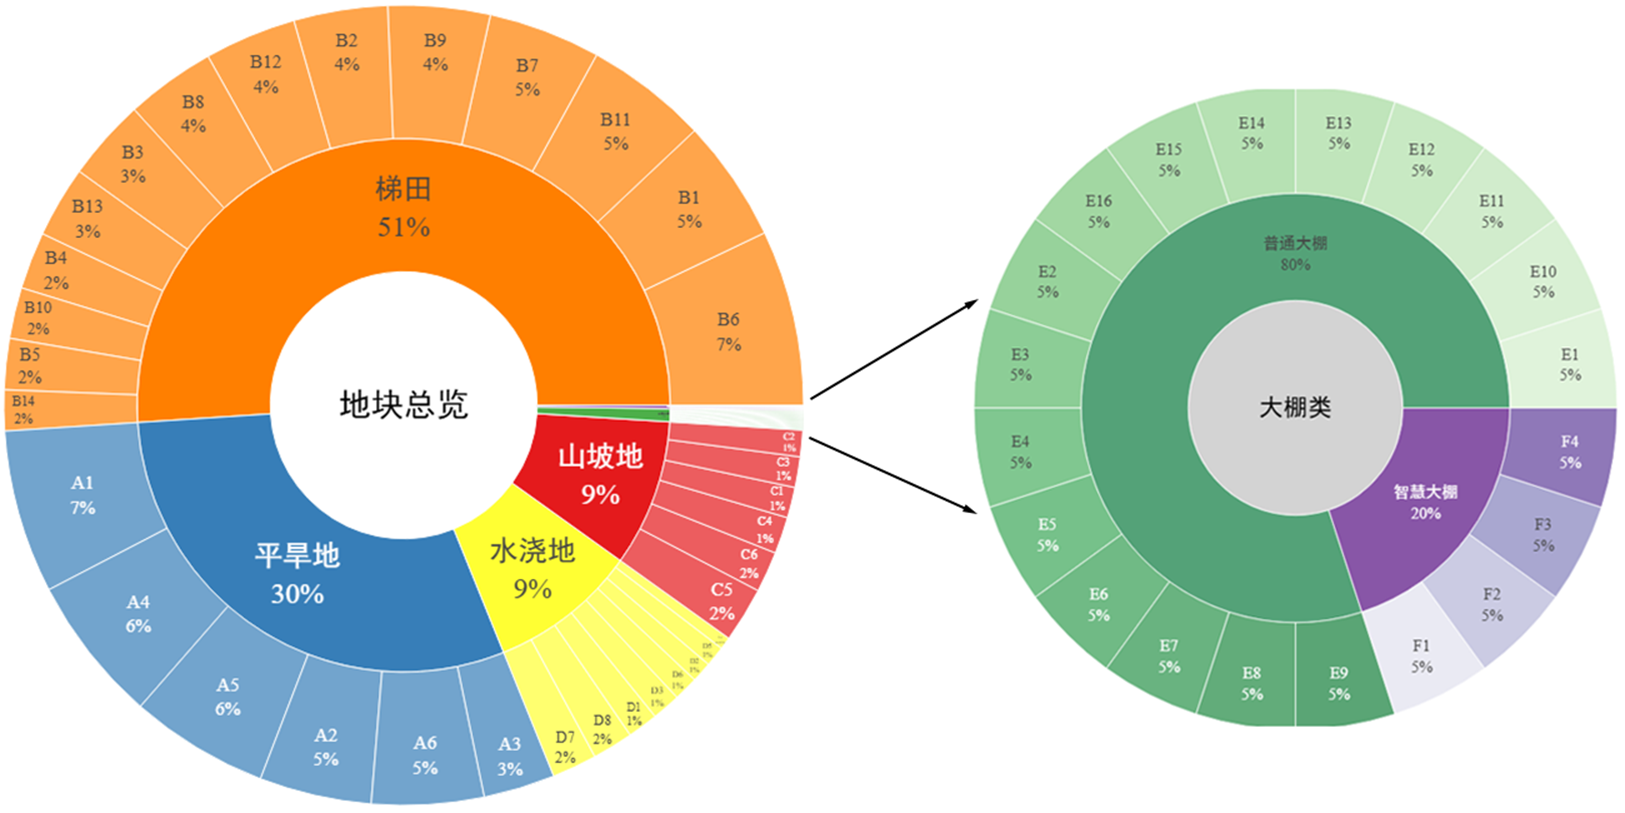
\includegraphics[width=0.8\textwidth]{../figures/0_1.png}
	\caption{露天耕地结构(左)与大棚耕地结构(右)分布图}
	\label{fig:land_structure}
\end{figure}

\subsection{农作物种植现状与经济效益分析}

为建立后续模型的经济基准,我们对2023年的农作物生产数据进行分析。图\ref{fig:production_rank}依据总产量对2023年种植的各类作物进行排序,揭示了当前农业生产的整体格局。小麦、玉米等粮食作物在总产量上占据绝对主导地位,是维系该乡村农业经济的“压舱石”。根据模型假设,2023年的各类作物产量被视为恰好满足市场需求的水平,因此这一产量数据为模型中的基准市场需求参数$Demand_j$的设定提供了直接依据。

\begin{figure}[h]
	\centering
	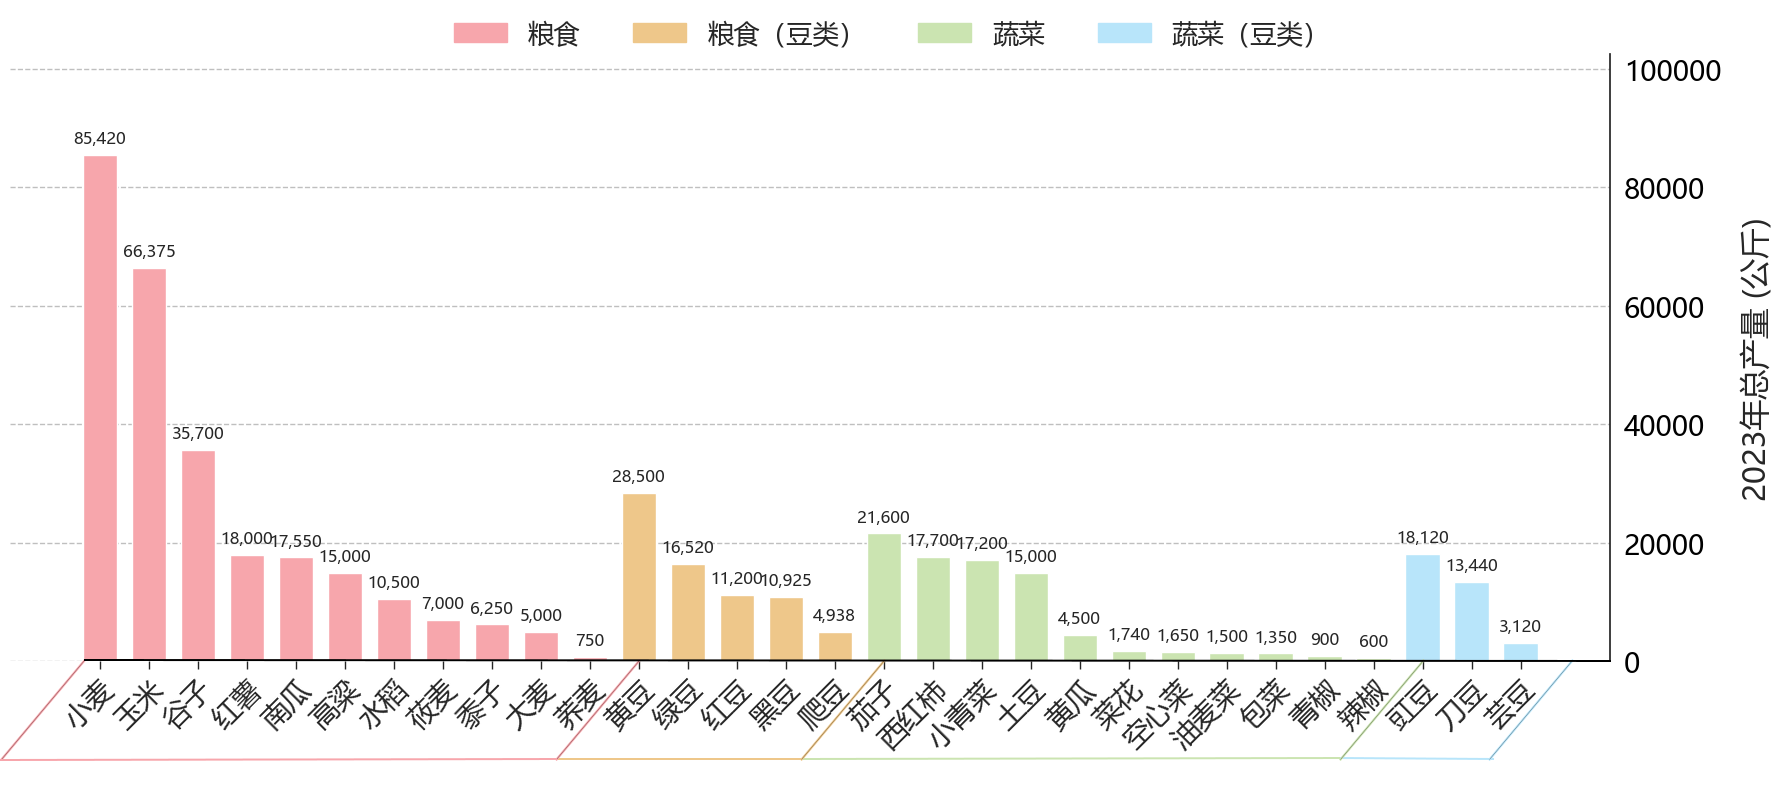
\includegraphics[width=0.9\textwidth]{../figures/0_2.png}
	\caption{2023年各类农作物总产量排名}
	\label{fig:production_rank}
\end{figure}


经济效益是驱动种植决策的核心。我们结合附件数据核算了各类作物的亩均净利润(见图\ref{fig:profit_per_mu})。分析发现,作物间的盈利能力存在巨大差异。羊肚菌、大白菜等经济作物展现出极高的亩均利润,而粮食作物的单位利润则偏低。这种显著的利润分化揭示了该乡村面临的经典经济学权衡:高利润经济作物如同高风险高回报的“成长股”,而粮食作物则像是收益稳定、保障基本盘的“债券”。因此,最优种植策略的本质,可以类比为在现代投资组合理论的指导下,构建一个平衡风险与收益的、最优化的“农业资产包”。

\begin{figure}[htbp]
	\centering
	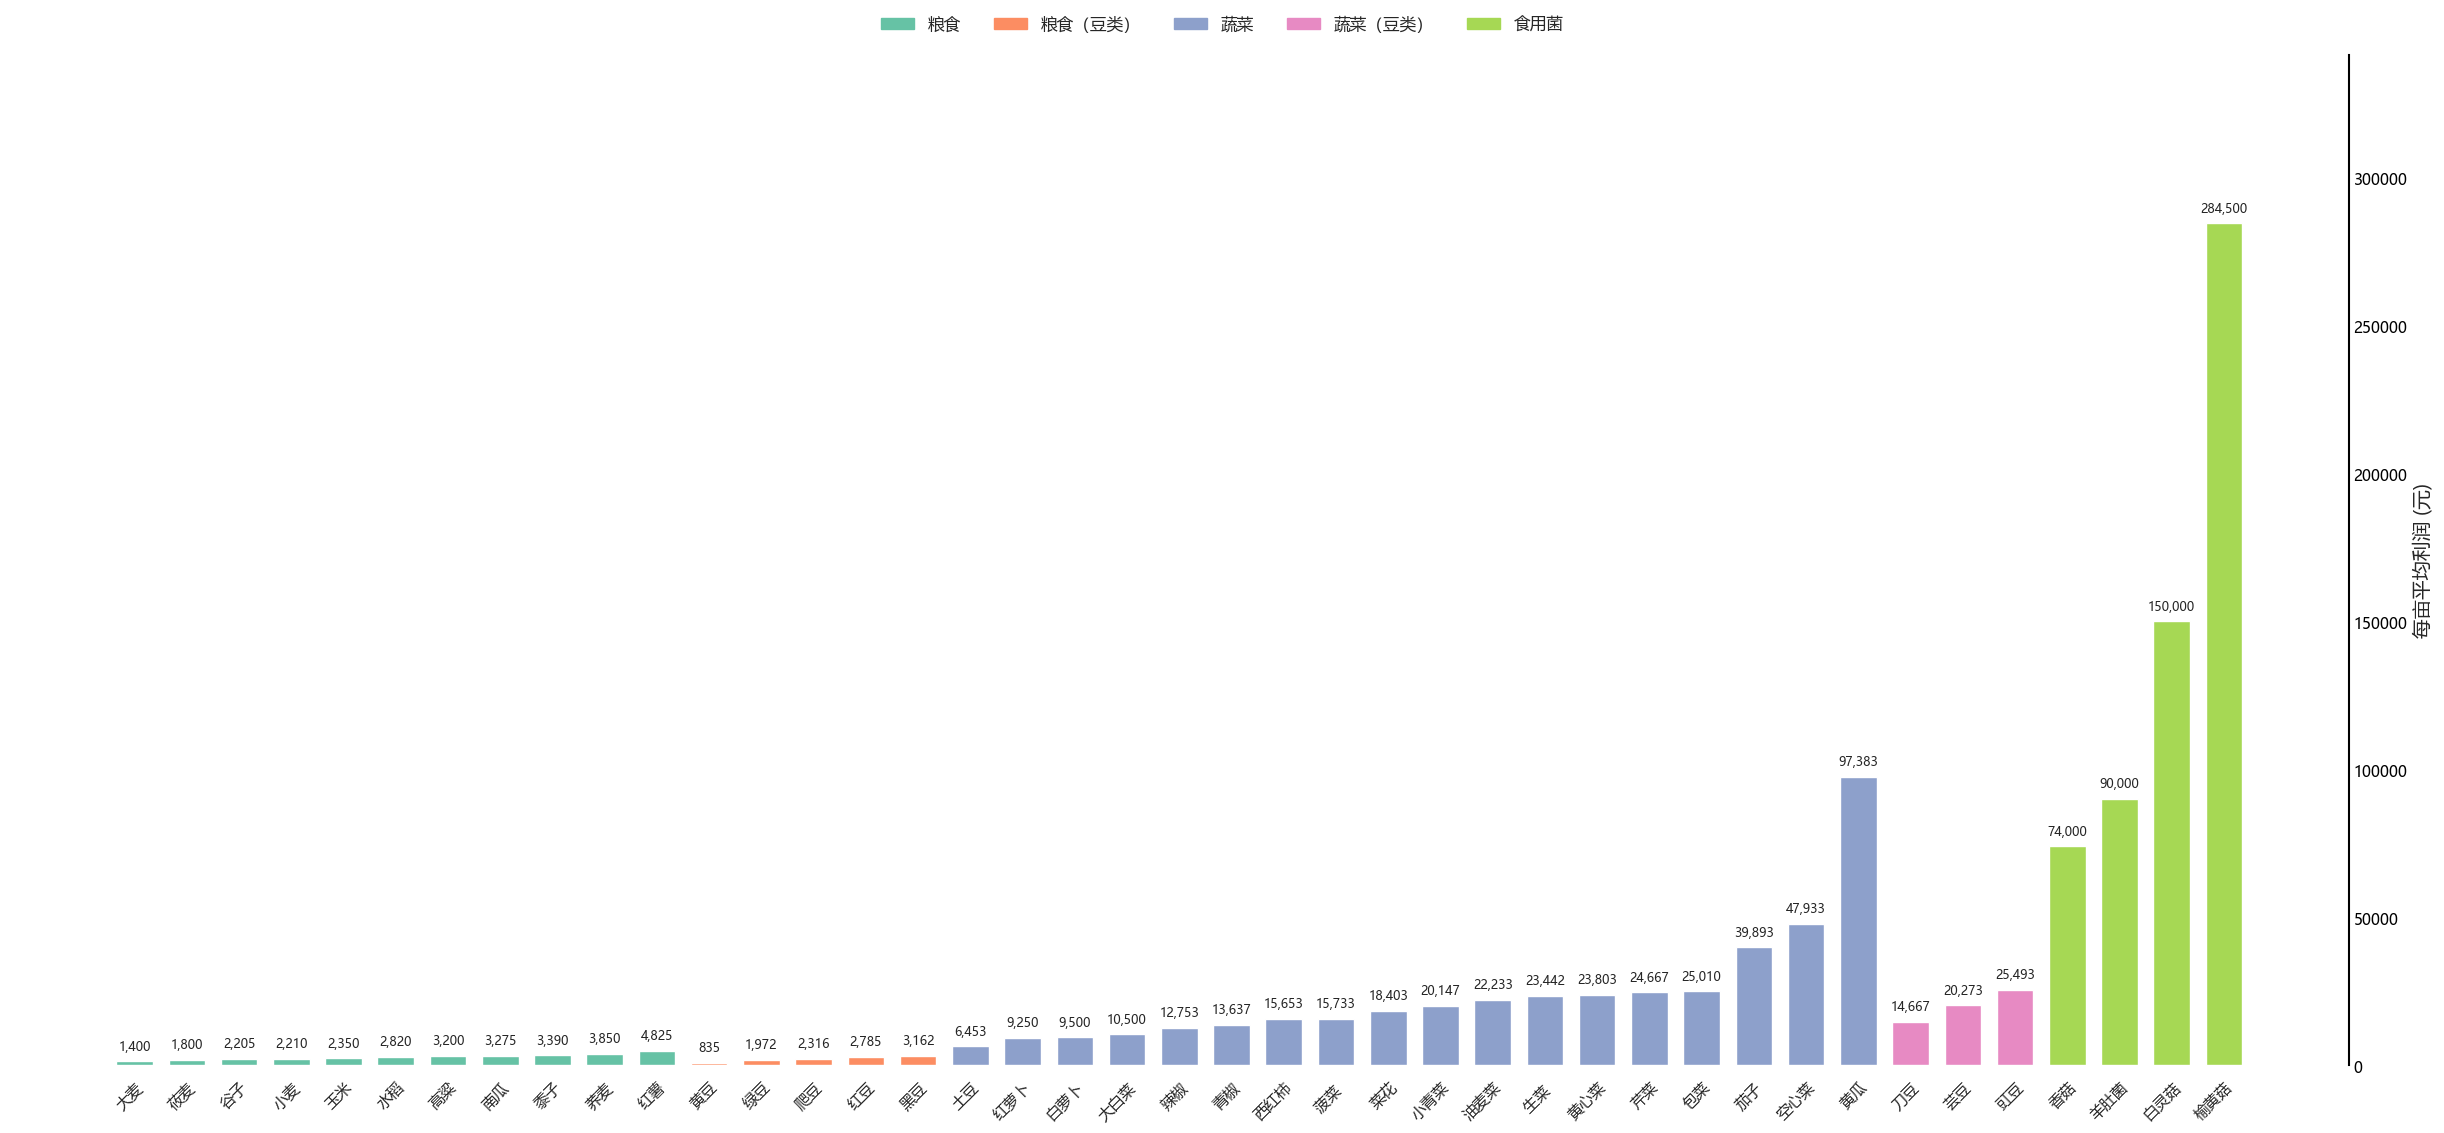
\includegraphics[width=0.9\textwidth]{../figures/0_3.png}
	\caption{各类农作物亩均净利润对比分析}
	\label{fig:profit_per_mu}
\end{figure}